\documentclass[10pt]{article}
\usepackage{commands}


\begin{document}
%Course webpage: https://phas.ubc.ca/~seme/516/
\begin{tcolorbox}
  \begin{center}
  \begin{Large}
    \textbf{PHYS 516 (Statical Mechanics) Notes} \\
    \vspace{5pt}
  \end{Large}
  \begin{large}
        Rio Weil \\
\vspace{5pt}
    \emph{This document was typeset on \today}
  \end{large}
  \end{center}
\end{tcolorbox}
% Email: gordonws@phas.ubc.ca
% Office: Henn 344
% Webpage: https://phas.ubc.ca/~seme/516/


\begin{center}
  \textbf{Introduction:}

  This is a set of lecture notes taken from UBC's PHYS 516 (Graduate Statistical Mechanics) course, taught by Dr. Gordon Semenoff. The course covers fundamentals of statistical mechanics, phase transitions and critical exponents, $D = 1,2,3$ Ising models, mean field theory, quantum field theory, universality, renormalization, and elementary conformal field theory. If any errors are found in the notes, feel free to email me at \href{mailto:ryoheiweil@phas.ubc.ca}{ryoheiweil@phas.ubc.ca}.
\end{center}
\addtocontents{toc}{\protect\hypertarget{toc}{}}
\tableofcontents

\newpage
\section{Introduction, Statistical Mechanics Review}

\subsection{Overview}
This course centers around critical phenomena and phase transitions (primarily in magnetic systems/the Ising model) - PHYS 403 is a more comprehensive overview of the field, this is more specialized. We will discuss models that are analytically solvable (or almost), some renormalization group methods, some conformal field theory and the conformal bootstrap method.

We will begin with a review of some basic statistical mechanics. In a nutshell, statistical mechanics is the application of probability theory to a physical system - typically, with a large number of degrees of freedom as this is the limit where the application is useful. Perhaps saying probability theory is a bit reaching, though - the probability involved is pretty minimal (lots of counting, not a ton of measure theory). It is worth noting that (much like other fields of physics) there are very few systems that are analytically solvable; most systems require the application of approximate techniques.

\subsection{Canonical Ensemble}
There are various places to begin this discussion; let's start by discussing the canonical ensemble. Let us consider a physical system, which has an array of possible states. Let us assume that it is characterized by energies $E_a$, and the energy can take up one out of a list of possible values $E_1, E_2, E_3, \ldots$. Given the conservation of energy for a closed system, this is a reasonable way to characterize a state (and given one of our goals of doing thermodynamics with our system, this is a useful quantity). Let us not say too much more about the system - other than perhaps the fact that the energy has a lower bound (but not necessarily an upper bound), and that the energies are ordered. Further, for now let us assume that the energies are discrete - this is of course not true in general (there exist systems for which energy is a continuum, and there we will have to use some kind of binning procedure), but let us assume this simplification for now.

So, how do we make the canonical ensemble? We take $\N$ copies of the system, with various energies, so that $\mathcal{E} = \sum_{i=1}^{\N} E_i$ is the total energy. The $\N$ copies of the system are weakly coupled to each other. This means that energy can flow between the systems, but also that (since the coupling is weak) when we calculate the total energy we can neglect the interaction energies between the systems. In other ensembles, other things that are not the energy can be exchanged (e.g. particles in the grand canonical ensemble).

\begin{figure}[htbp]
    \centering
    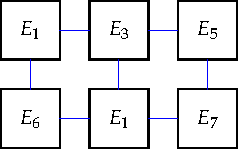
\includegraphics[]{Images/fig-canonicalensemble.pdf}
    
    \caption{Cartoon of the Canonical Ensemble - we consider $\N$ ($= 6$ here) copies of a system, and weakly couple them such that they can exchange energy.}
    \label{fig-canonicalensemble}
\end{figure}

In state of the ensemble is specified by the number of systems with a given energy, i.e. there are $n_1$ systems with energy $E_1$, $n_2$ systems with energy $E_2$, and so on. The total energy is then given by:
\begin{equation}
    \mathcal{E} = \sum_{a} n_a E_a
\end{equation}
and the number of systems in the ensemble is given by:
\begin{equation}
    \N = \sum_a n_a
\end{equation}

\subsection{Fundamental Postulate - Equal a Priori Probability}
To do statistical mechanics, we require a fundamental postulate - namely, an ``equal a priori probability''. This says that every distinct configuration of the ensemble is equally likely, subject to the total energy and number constraints. Physically, this means that the systems in the ensemble in time are flipping around the possible energy states (in a way that the total energy of the ensemble is conserved). The most probable configuration is the state in which the system spends the most time.

There are other versions of this; we can for example divide a system up in space, and then a spatial average will yield the most probable distribution.

What we look for (since the system visits every possible configuration equally) is the configuration which can be made in the most number of ways. And this is really the only probability theory we have to worry about here; counting up the number of ways to yield a given configuration of the ensemble. So, we ask how many ways are there to make the state $(n_1, n_2, \ldots)$? Let us derive this. Starting with the systems with energy $E_1$, we have:
\begin{equation}
    \N(\N-1) \ldots (\N - n_1 + 1)
\end{equation}
ways to have $n_1$ systems with energy $E_1$ (this is obtained by considering there are $\N$ systems to choose to have energy $E_1$, then $\N - 1$ systems, and so on until all $n_1$ systems have been chosen). But this is overcounting because we don't care about the order, so really we require to divide this by $n_1!$:
\begin{equation}
    \frac{\N(\N-1) \ldots (\N - n_1 + 1)}{n_1!}
\end{equation}
and we continue with $n_2, n_3$ and so on until everything is full:
\begin{equation}
    \frac{\N(\N-1) \ldots (\N - n_1 + 1)}{n_1!} \frac{(\N - n_1) \ldots (\N - n_1 - n_2 + 1)}{n_2!} \ldots = \frac{\N!}{n_1!n_2!\ldots}
\end{equation}
So, the most probable state of the system is that for which the above is maximized; in other words, we maximize it subject to $\sum_{a} n_a = \N$ and $\sum_a n_a E_a = \mathcal{E}$. This is a optimization problem with constraints - this may remind you of Lagrange multipliers which you have seen in classical mechanics. There is an apparent difficulty here in the fact that our numbers are discrete, but we'll get around it. To start, let us take the logarithm of the expression; we can maximize the logarithm of it instead of the original expression, and this is legal as the logarithm is monotonic (this is also a common trick done in machine learning and maximum likelihood estimation). The technique of Lagrange multipliers tells us that the expression of our interest is:
\begin{equation}\label{eq-Lagrangemults}
    \ln(\frac{\N!}{n_1!n_2! \ldots}) + \beta\left(\sum_a n_a E_a - \mathcal{E}\right) + \gamma\left(\sum_a n_a - \N\right)
\end{equation}
it would be nice to be able to use calculus techniques to solve this problem; to this end let us work in the regime of large $\N$ such that we can make the continuum approximation. At first this might seem like a poor assumption; after all after we saturate $\mathcal{E}$ all of the $n_a$s past that point better not be large, but instead zero! To get around this we could assume some kind of cutoff to the energies. Of course there is still a decaying tail to the $n_a$s, but these turn out to not be a problem.

In any case, let us suppose that we can approximate $\N$ large. Then, we can apply Stirling's formula:
\begin{equation}\label{eq-Stirling}
    \ln \N! \approx \N\ln \N - \N.
\end{equation}

\subsection{Interlude - Deriving Stirling's Formula}
We start by writing down an integral expression for the factorial:
\begin{equation}
    \N! = \int_0^\infty dx x^\N e^{-x}
\end{equation}
we solve this via a saddle point technique of replacing the integrand with its maximum value; taking the derivative of the integrand and setting it to zero, we have:
\begin{equation}
    \N x^{\N-1}e^{-x} - x^\N e^{-x} = 0
\end{equation}
which is maximized at $x = \N$. so, the approximate value of the factorial is:
\begin{equation}
    \N! \approx \N^\N e^{-\N}
\end{equation}
and taking logarithms we get Eq. \eqref{eq-Stirling}. This technique also gives us a way of considering corrections to Stirling's formula by considering $x$ near $\N$ (the next order corrections to $\ln \N!$ are $O(\log \N)$, for example).

Another quick and dirty way to derive the formula (that doesn't give a nice way to study corrections, but gives us the leading terms that we want). Using the definition of the factorial and laws of logarithms, we have:
\begin{equation}
    \ln \N! = \sum_{j=1}^\N \ln j
\end{equation}
now approximating the sum as an integral:
\begin{equation}
    \ln\N! \approx \int_1^\N dj \ln j = \N\ln\N - \N + 1
\end{equation}
in the large $\N$ limit we may neglect the $+1$, and we (again) obtain Stirling's formula.

\subsection{Deriving the Boltzmann Distribution}
Applying Stirling's Formula, Eq. \eqref{eq-Lagrangemults} becomes:
\begin{equation}
    \N\ln\N - \N - \sum_a(n_a \ln n_a - n_a) + \beta(\sum_a E_a n_a - \mathcal{E}) + \gamma(\sum_a n_a - \N) = \N\left(\sum_a(-\rho_a \ln \rho_a) + \beta(\sum_a \rho_a E_a - U) + \gamma(\sum_a \rho_a - 1)\right)
\end{equation}
where we define $\rho_a = \frac{n_a}{N}$ and the second expression follows by algebra. Now, since $\rho_a$ varies slowly, we may use techniques of calculus and take a derivative of the above expression and set it to zero. The $\rho_a$ equation reads:
\begin{equation}
    -\ln \rho_a - 1 + \beta E_a + \gamma = 0
\end{equation}
we also take derivatives by $\beta, \gamma$ and set them to zero (as we do with the Lagrange multiplier technique):
\begin{equation}
    \sum_a \rho_a E_a = U
\end{equation}
\begin{equation}
    \sum_a \rho_a = 1
\end{equation}
Let us rearrange the first equation, which has solution:
\begin{equation}
    \rho_a = e^{\beta E_a + \gamma - 1}
\end{equation}
we don't solve the second one, but the third one gives us:
\begin{equation}
    \rho_a = \frac{e^{\beta E_a}}{\sum_a e^{\beta E_a}}
\end{equation}
Note that the $e^{\gamma - 1}$ goes away when we solve the third equation. It would have been wise to choose $\beta$ with the other sign to start with. As we have derived things here, things only make sense if $\beta < 0$. We note that we have derived the ever-famous partition function:
\begin{equation}
    Z = \sum_a e^{\beta E_a}
\end{equation}

So, we have solved for the most likely distribution $\rho_a$; this is the known as the ``Boltzmann distribution''. We have not solved explicitly for $\beta$, but the second equation is formally unsolvable, and we will find a nice interpretation for $\beta$ anyway (as the familiar $\beta = -\frac{1}{k_B T}$). 

\subsection{Example: Two-level system}
We really have not done any physics at all here; but, we have completely generically found the most probable distribution. Let us try applying this to a two-level system and see how good our result is. Particles can have two (spin) states, $\uparrow$ and $\downarrow$. Let us assume we have two particles, and let us assume all orientations of the spins have the same energy. We can just enumerate all the states, and characterize the system by the net magnetization $m = \# \uparrow - \# \downarrow$. We have the four states $\uparrow \uparrow$ with $m = 2$, $\downarrow \downarrow$ with $m = -2$, $\uparrow\downarrow$ and $\downarrow \uparrow$ with $m = 0$. Here, the technique of most probable distribution is quite poor - there is a very good probability that the system is actually ferromagnetic (in fact half of the time) even though the most probable distribution is that the system is unmagnetized. However, we are able to see that unmagnetized is the most probable distribution, and in fact this is true for any number of particles.

So, let's consider generically $N$ particles (note - let us assume that $N$ is even so we can avoid frustration; if $N$ is odd then there exists no configuration with zero magnetization). With $N$ particles, the number of states with $n$ spins up (from which we can obtain the magnetization as $m = n - (N - n) = 2n - N$) is $\frac{N!}{n!(N-n)!}$ of $2^n$ total possible states.

If we then plot $\ln \frac{N!}{n!(N-n)!}$ (making the continuum approximation), we find:

\begin{figure}[htbp]
    \centering

    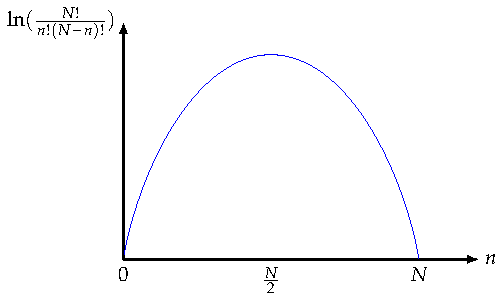
\includegraphics[]{Images/fig-TLSstatecounting.pdf}
    
    \caption{Plot of (continuum approximation) $\ln\frac{N!}{n!(N-n)!}$ as a function of number of spin-up spins $n$. We see the maximum at $n = N/2$ (zero magnetization).}
    \label{fig-TLSstatecounting}
\end{figure}

so indeed the state with $n = N/2$ spins up (and $n = N/2$ spins down) - the state with total magnetization $m = 0$ is the most probable state. It is also valuable to ask what fraction of the total number of states is the most likely distribution. This is simply obtained by taking the number of states with $n = N/2$ and dividing by the total $2^n$:
\begin{equation}
    \frac{N!}{(N/2)!(N/2)!} \frac{1}{2^{n}}
\end{equation}
We find that (using Stirling's formula that):
\begin{equation}
    \ln( \frac{N!}{(N/2)!(N/2)!} \frac{1}{2^{N}}) = 0 + \frac{\ln N}{N}
\end{equation}
so in the $N \to \infty$ limit, $\frac{N!}{(N/2)!(N/2)!} \frac{1}{2^{N}} \approx 1$ to leading order, so the proportion of the most likely distribution to total states of the system is one (with corrections given by the successive terms).
\newpage
\section{Free Energy, Ideal Gas, and the Grand Canonical Ensemble}

\subsection{Thermodynamic Interpretation, Energy, and Free Energy}
Last time, we looked at the canonical ensemble. We derived the most probable distribution:
\begin{equation}
    \rho_a = \frac{e^{-\beta E_a}}{\sum_a e^{-\beta E_a}}
\end{equation}
and found the partition function:
\begin{equation}
    Z = \sum_a e^{-\beta E_a}.
\end{equation}
We argue that this already has a nice thermodynamic interpretation. This comes about if we look at the logarithm of the partition function:
\begin{equation}
    F = -\frac{1}{\beta}\ln Z = -\frac{1}{\beta}\ln \sum_a e^{-\beta E_a}
\end{equation}
Note that if there was only one energy level, then this would immediately just be the energy - in general the energy we calculate as the expectation value:
\begin{equation}
    U = \frac{\sum_a E_a e^{-\beta E_a}}{\sum_a e^{-\beta E_a}}
\end{equation}
How does $F$ relate to $U$? Let us write:
\begin{equation}
    F = U + \left(-\frac{1}{\beta}\ln \sum_a e^{-\beta E_a} - \frac{\sum_a E_a e^{-\beta E_a}}{\sum_a e^{-\beta E_a}}\right)
\end{equation}
Let us call $e^{-\beta E_a} = Z \rho_a$ and write $E_a = -\frac{1}{\beta}\ln Z - \frac{1}{\beta}\ln \rho_a$. Then, rewriting the above expression, we find:
\begin{equation}
    F = U - \frac{1}{\beta}\sum_a \rho_a \ln \rho_a.
\end{equation}
The second term should be familiar to anyone with an information theory background - $S_{VN} = \sum_a \rho_a \ln \rho_a$ is known as the von Neumann entropy. It is the entropy of the distribution - a measure of how little we know about the system when we have the distribution $\rho_a$. It is minimized if one of the $\rho$s is one and the others are zero, as the entropy is zero (then we know exactly what the system is). It is maximized if all of the $\rho$s are constant (because then we know nothing about the system). If we are willing to accept that the von Neumann entropy is equal to the thermal entropy up to a constant:
\begin{equation}
    S = k_B S_{VN}
\end{equation}
where $k_B$ is Boltzmann's constant. Then, we obtain:
\begin{equation}
    F = U - \frac{1}{\beta}\frac{S}{k_B}
\end{equation}
which closely resembles:
\begin{equation}
    F = U - TS. 
\end{equation}
where $T$ is the temperature (if we interpret $\beta = \frac{1}{k_B T}$). This is the familiar thermodynamic expression for the Helmholtz free energy.

This is not the historical order in which things are done - historically the microcanonical viewpoint (due to Boltzmann) came first, but this requires the system to be thermodynamic.

\subsection{Example - System of weakly interacting non-relativistic particles}
Let us assume we have a collection of $N$ weakly interacting non-relativistic particles of mass $m$, which obey the laws of classical mechanics. A state of such a system will just be the specifications of the positions and velocity (or momenta) of all the particles (mathematically, this is because Newton's second law is a second-order ODE so we require two boundary conditions to specify the state). We can write the state as a collection of these values $\set{\v{q}_1, \v{p}_1, \ldots, \v{q}_n, \v{p}_n}$ The energy is then given by the Hamiltonian:
\begin{equation}
    H = \sum_k \frac{\v{p}_k^2}{2m}
\end{equation}
Note we assume that the masses of the particles are the same and all attributes of the particles (other than position or momentum) are identical - note that in the context of classical mechanics this does not make the particles indistinguishable - we can keep track of them. This is in contrast to quantum statistical mechanics, where particles are truly indistinguishable and are either fermions or bosons.

We can construct the partition function for this system:
\begin{equation}
    Z = \int d\v{q}_1 d\v{p}_1 \ldots d\v{q}_n d\v{p}_n e^{-\beta H}
\end{equation}
this looks reasonable, but there are a couple things wrong with this. One problem - $Z$ has dimensions; this is problematic if we want to take functions of it (e.g. logarithms to get the free energy). To deal with this problem, we just divide it by a number that gets rid of the dimensions:
\begin{equation}
    Z = \frac{1}{(2\pi \hbar)^{3N}}\int d\v{q}_1 d\v{p}_1 \ldots d\v{q}_n d\v{p}_n e^{-\beta H}
\end{equation}
$\hbar$ we pretty much pulled out of a hat here, but we require something with the dimensions of angular momentum to place there. Let's now do the integral. Let's assume that our particles move in infinite 3-D Euclidean space; we can then write $\int d\v{q}_i = V$ (the volume) as $H$ does not depend on the positions. Further, all momentum integrals are equivalent, so let us write it as the product of momentum integrals:
\begin{equation}
    Z = \frac{V^N}{(2\pi \hbar)^{3N}}\left(\int dp e^{-\frac{\beta}{2m}\v{p}^2}\right)^{3N}
\end{equation}
We go into polar coordinates to solve this Gaussian integral:
\begin{equation}
    \left(\int dp\right)^{3N} \to \left(\int d^2p\right)^{\frac{3N}{2}} \to \left(\int \frac{d\phi pdp}{2}\right)^{\frac{3N}{2}}
\end{equation}
which yields:
\begin{equation}
    Z = \frac{V^N}{(2\pi \hbar)^{3N}} \left(\frac{2\pi m}{\beta}\right)^{\frac{3N}{2}} = V^N\left(\frac{mk_B T}{2\pi \hbar^2}\right)^{\frac{3N}{2}}
\end{equation}
The Helmholtz free energy is then:
\begin{equation}
    F[T, V, N] = -k_B T N\ln \left[V\left(\frac{mk_B T}{2\pi \hbar^2}\right)^{3/2}\right]
\end{equation}
This system should be truly thermodynamic (as we can take the system to be large), so this should work - we will see in a moment that unfortunately, it does not!

Recall thermodynamic differential relation:
\begin{equation}
    dF = -S dT + \mu dN - P dV
\end{equation}
So the entropy is:
\begin{equation}
    S = \left.-\dpd{F}{T}\right|_{N, V}
\end{equation}
the chemical potential is:
\begin{equation}
    \mu = \left.\dpd{F}{N}\right|_{T, V}
\end{equation}
and the pressure is:
\begin{equation}
    P = \left.-\dpd{F}{V}\right|_{T, N}
\end{equation}
so we can go to town and calculate some quantities. For example
the pressure we can calculate to be:
\begin{equation}
    P = \frac{N k_B T}{V}
\end{equation}
which is the ideal gas law! Big success (the other quantities will not be as successful...)! The chemical potential we can calculate to be:
\begin{equation}
    \mu = -k_B T\ln\left(V\left(\frac{mk_B T}{2\pi \hbar^2}\right)^{3/2}\right)
\end{equation}
The entropy we calculate to be:
\begin{equation}
    S = \frac{3}{2}k_B N + k_B N\ln\left(V\left(\frac{m k_B T}{2\pi \hbar^2}\right)^{3/2}\right)
\end{equation}
We can calculate the energy to be:
\begin{equation}
    U = F + TS = \frac{3}{2}N k_B T
\end{equation}
which is again a beautiful formula (and the correct result). However, we should talk about why the formulas for $\mu, S$ are wrong. They do not have the correct extensivity properties. Concretely, if one considers two identical volumes of ideal gas separated by a partition, removing and re-inserting the partition should be reversible. However, a calculation of the entropy change shows that removing the partition leads to an increase in entropy of $2k_B N \ln 2$; contradiction. So we're a failure. But we're also clever, and can try to fix it. We introduce a factor of $\frac{1}{N!}$ into the partition function. This introduces a factor of $\frac{1}{N}$ into the logarithm in the free energy expression, which ends up correcting things. This was originally a fudge factor fix, but it turns out to be quite deep - namely, we have overcounted the states in the system somehow, and the $\frac{1}{N!}$ corrects for this. This hints to classical mechanics being problematic (quantum statistics fixes this with indistinguishability). 

But let's try taking $Z \to \frac{1}{N!}Z$ (we are exploring what is known as Maxwell-Boltzmann statistics). Then with Stirling's formula:
\begin{equation}
    \ln N! \approx N\ln N - N = \ln \left(\frac{N}{e}\right)^N
\end{equation}
Then the free energy becomes:
\begin{equation}
    F[T, N, V] = -k_B T\ln\left[\frac{eV}{N}\left(\frac{mk_B T}{2\pi \hbar^2}\right)^{3/2}\right]
\end{equation}
and now we see that $F$ has the correct scaling properties so things have been fixed. If we now recalculate quantities, $P, U$ stay the same (as beautiful as they were):
\begin{equation}
    PV = Nk_B T
\end{equation}
\begin{equation}
    \frac{U}{N} = \frac{3}{2}k_B T
\end{equation}

And now the entropy is fixed up as well:
\begin{equation}
    S = \frac{3}{2}k_B N + k_B N\ln\left(\frac{eV}{N}\left(\frac{mk_B T}{2\pi\hbar^2}\right)^{3/2}\right)
\end{equation}
and this is known as the \emph{Sackur-Tetrode equation}.

Before we go on - there are other ensembles we could have used, e.g. the grand canonical ensembles where the subsystems are allowed to exchange particles as well as energy. We need this as this one is the easier one to use when we consider quantum statistics. So in a way, Maxwell-Boltzmann statistics assumes the distribution is completely symmetric in the particles, but it is blind to how the wavefunction changes - if we take the distribution to be $\rho = \psi^\dag \psi$, it assumes that each permutation comes out to be symmetric. But is not actually completely correct as in QM we impose the proper statistics on the wavefunctions, rather than the density.

\subsection{Grand Canonical Ensemble}
The logic follows exactly the same as the Canonical ensemble, with the only difference that we allow for the particle number to change. Suppose a system has $N_a$ particles in state $a$, and energy $E_a$. We define $n_a$ to be the number of systems in the ensemble in state $a$. We have some constraints:
\begin{equation}
    \sum_a n_a = \mathcal{N}
\end{equation}
\begin{equation}
    \sum_a n_a E_a = \mathcal{E} = \mathcal{N}U
\end{equation} 
\begin{equation}
    \sum_a n_a N_a = \mathcal{N}N
\end{equation}
in the above, $U$ is the average energy and $N$ is the average number of particles. This differs from what we had before by one equation. We want to find the most probable distribution; for this the mathematics is exactly the same, just with one more Lagrange multiplier. We maximize:
\begin{equation}
    \ln \frac{\mathcal{N}!}{\prod_a n_a !} + \beta(U\mathcal{N} - \sum_a n_a E_a) + \alpha\left(N\mathcal{N} - \sum_a n_a N_a\right) + \gamma\left(\mathcal{N} - \sum_a n_a\right)
\end{equation}
The argument is basically identical to what we did to calculate $\rho_a$ for the canonical ensemble. We solve the first and last equations for $\rho_a$ and leave the other two unsolved (they will be thermodynamic quantities we can interpret). After the dust settles, we end up with:
\begin{equation}
    \rho_a = \frac{e^{-\beta E_a - \alpha N_a}}{\sum_a e^{-\beta E_a - \alpha N_a}}
\end{equation}
Our grand canonical partition function is:
\begin{equation}
    \mathcal{Z} = \sum_a e^{-\beta E_a - \alpha N_a}
\end{equation}
If we identify:
\begin{equation}
    \Phi = -k_B T \ln \mathcal{Z}
\end{equation}
with the grand canonical free energy, and go through a similar procedure of identifying the Von Neumann entropy with the thermodynamic entropy (and an identification to relate $\alpha$ with the chemical potential), we obtain:
\begin{equation}
    \beta = -\frac{1}{k_B T}, \quad \alpha = -\frac{\mu}{k_B T}.
\end{equation}
The grand canonical free energy now no longer depends on the number of particles, but on the chemical potential. It is however related to the Helmholtz free energy via a Legendre transform:
\begin{equation}
    \Phi[T, \mu, V] = F - \mu \mathcal{N}
\end{equation}
If we did things correctly, working with the grand canonical free energy vs. the Helmholtz free energy should yield the same answers. If we recall the canonical partition function for the weakly interacting gas, we had a dependence on the particle number $N$ (note - NOT the average number of particles in the systems of the ensemble, but here really the number of particles in the ideal gas. Sorry for the overload of notation). We can sum over $N$ to get the grand canonical partition function. We can then go through and see if we obtain the same results (and we will). We had:
\begin{equation}
    Z[T, N, V] = \frac{1}{N!}V^N\left(\frac{mk_B T}{2\pi \hbar^2}\right)^{\frac{3N}{2}}
\end{equation}
note the inclusion of the $\frac{1}{N!}$ factor so things end up correct. The grand canonical partition function is then:
\begin{equation}
    \mathcal{Z}[T, \mu, V] = \sum_N e^{\frac{\mu}{k_B T}N}Z[T, N, V]
\end{equation}
this is an easy sum because its just $\sum_N \frac{1}{N!}x^N$; hopefully this is familiar as just an exponential:
\begin{equation}
    \mathcal{Z}[T, \mu, V] = e^{V\left(\frac{mk_B T}{2\pi \hbar^2}\right)^{3/2}e^{\frac{\mu}{k_B T}}}
\end{equation}
so our prediction for the grand canonical free energy is:
\begin{equation}
    \Phi = -k_B T \ln \mathcal{Z} = -k_B TV\left(\frac{mk_B T}{2\pi \hbar^2}\right)^{3/2}e^{\frac{\mu}{k_B T}}
\end{equation}
and we can go through the song and dance to obtain the quantities that we solved for using the canonical ensemble.
\newpage
\section{Microcanonical Ensemble, Quantum Statistical Mechanics}
We have spent two lectures discussing the canonical ensemble and grand canonical ensemble - in this setting we have discussed the classical perfect gas. We have one more to discuss; the microcanonical ensemble.

\subsection{Review of the Canonical Ensemble}
The canonical ensemble is a way to find the likelihood that a system is in a particular state; we found the most likely distribution:
\begin{equation}
    \rho_a = \frac{e^{-\beta E_a}}{\sum_a e^{-\beta E_a}}
\end{equation}
with $\beta = \frac{1}{k_B T}$. In deriving this we made some assumptions; for example the fact that the system was able to visit different energy states (this may not be true, e.g., if the system obeys some conservation law). In the setting of the perfect gas, we assumed that the particles were weakly interacting so they could exchange energy and visit different energy states (but weakly so we did not have to consider the interaction very carefully) - if the particles were completely free, they could not change their state (the momenta of all the particles would be fixed). We explored this distribution in the context of an ensemble of two-level systems; for two spins, we found that this was only a good description $\sim 50\%$ of the time, but as we increase $N$ this estimate gets better and better.

\subsection{Microcanonical Ensemble}
The accuracy of the canonical ensemble only depended on the size of the ensemble - if something is not accurate enough, just look at a larger system. Essentially, a given subsystem sees the rest of the system as a heat bath/reservoir, and the estimate will get better as we increase the size of the heat bath. But we might ask - how well is the system described if we assume the system takes the most likely state? Roughly, the system takes the state such that $E^\nu e^{-\beta E}$ is maximized (those with a condensed matter background will be familiar with this sort of expression; the Boltzmann distribution times the density of states).

Concretely, we say:
\begin{equation}
    \rho_a = \begin{cases}
        1 & a: E_a = U
        \\ 0 & \text{otherwise}
    \end{cases}
\end{equation}
This looks extremely crude; it doesn't always work (e.g. the system needs to be highly degenerate) but for most normal things, it does. Let's reason out why. We consider the heat capacity:
\begin{equation}
    C = \left.\dpd{U}{T}\right|_{\ldots} \sim V c
\end{equation}
where $C$ (the total heat capacity) scales with volume (times the per-volume heat capacity/specific heat capacity $c$).

In the canonical approach, $U$ is the average of the energy:
\begin{equation}
    U = \sum_a\frac{ E_a e^{-\beta E_a}}{\sum_a e^{-\beta E_a}} = \avg{E}
\end{equation}
We can write the heat capacity as:
\begin{equation}
    C = \dpd{U}{T} = \frac{1}{k_B T^2}\Delta U^2
\end{equation}
where:
\begin{equation}
    \Delta U^2 = \sum_a \frac{E_a^2e^{-\beta E_a}}{\sum_a e^{-\beta E_a}} - \left(\frac{\sum_a E_a e^{-\beta E_a}}{\sum_a e^{-\beta E_a}}\right)^2 = \avg{E^2} - \avg{E}^2
\end{equation}
i.e. the variance in $E$. Note that both $C$ (and so $\Delta U^2$) and $U$ scale with the volume of the system. Now, if we consider the variance of the energy:
\begin{equation}
    \sqrt{\frac{\Delta U^2}{U^2}} \sim \frac{\sqrt{C}}{V} \sim \frac{1}{\sqrt{V}}
\end{equation}
so as we take $V \to \infty$, the variance in the energy becomes tiny. So the conclusion is that:
\begin{equation}
    \rho_a = \begin{cases}
        \frac{1}{D_a} & E_a = U
        \\ 0 & E_a \neq U
    \end{cases}
\end{equation}
(where $D_a$ is the degeneracy of $E_a$), is a reasonable distribution for (large) systems. 

Note that this can be a useful approach for classical statistical mechanics (for quantum statistical mechanics, the grand canonical ensemble is the best approach). We now have Boltzmann's formula\footnote{Carved on his headstone!} for the entropy in terms of the degeneracy of states:
\begin{equation}
    S = k_B \ln W
\end{equation}
where $W = D_a$. In Boltzmann's work, $W$ was known as the number of ways of making the system with energy $U$ (QM, and hence degeneracy, was not conceptualized at the time). This pre-dates Gibbs, and ensembles - it was a fantastic guess by Boltzmann, though it was not believed by the time.

\subsection{Ideal Gas - Microcanonical Ensemble Lens}
What we need to find is $W$, which in a sense is the partition function in this context. It depends on $U$ (and other quantities), and we obtain it by integrating $\delta(U - \sum_a \frac{\v{p}_a^2}{2m})$ over all possible positions and momenta:
\begin{equation}
    W[U] = \int d\v{q}_1d\v{p}_1 \ldots d\v{q}_Nd\v{p}_N \delta(U - \sum_a \frac{\v{p}_a^2}{2m}).
\end{equation}
There are a couple problems with this formula, one is namely the dimensionality (we want to plug this into a logarithm, so it must be dimensionless). Part of this is the same story as before; we add a phase space volume (fudge factor) of $\frac{1}{(2\pi\hbar)^{3N}}$ to cancel out the dimensions from the integral:
\begin{equation}
    W[U] = \int \frac{d\v{q}_1d\v{p}_1 \ldots d\v{q}_Nd\v{p}_N}{(2\pi\hbar)^{3N}} \delta(U - \sum_a \frac{\v{p}_a^2}{2m})
\end{equation}
Further, we need to cancel out the inverse energy that comes from the dirac delta function, so we add a $\delta U$ factor:
\begin{equation}
    W[U] = \int \frac{d\v{q}_1d\v{p}_1 \ldots d\v{q}_Nd\v{p}_N}{(2\pi\hbar)^{3N}} \delta U\delta(U - \sum_a \frac{\v{p}_a^2}{2m})
\end{equation} 
visually, one can imagine adding a sort of ``thickness'' of a shell of energy in phase space to the integral. This should go away whenever we start to do thermodynamics, though. Furthermore, we are overcounting states here again; so let us add a factor of $\frac{1}{N!}$ to compensate:
\begin{equation}
    W[U] = \frac{1}{N!}\int \frac{d\v{q}_1d\v{p}_1 \ldots d\v{q}_Nd\v{p}_N}{(2\pi\hbar)^{3N}} \delta U\delta(U - \sum_a \frac{\v{p}_a^2}{2m})
\end{equation}
The $\frac{1}{N!}\frac{1}{(2\pi\hbar)^{3N}}$ part of this is quantum, the rest is classical. Now, let's evaluate this. The position integrals are trivial; nothing in the integrand depends on volume, so we just get a factor of $V^N$. For the momentum integrals, we do a rescaling of the dirac delta function and then evaluate it, and also include the unit sphere factor in $3N$-dimensional Euclidean space:
\begin{equation}
    W[U] = \frac{1}{N!}V^N \frac{1}{(2\pi \hbar)^{3N}}\frac{\delta U}{U}(2mU)^{\frac{3N}{2}}\frac{2\pi^{3N/2}}{\Gamma(\frac{3N}{2})}
\end{equation}
Now, recall Stirling's formula $\ln N! = N\ln N - N$. The Gamma function is basically the factorial function, so $\ln \Gamma(x + 1) = x\ln x - x + \ldots$ (up to terms of order $O(\ln x)$). With this, we can clean up our expression for $W$:
\begin{equation}
    W[U, V, N] = \left(\frac{eV}{N}\left(\frac{2e}{3}\frac{mU/N}{2\pi \hbar^2}\right)^{3/2}\right)^{N}\frac{\delta U}{U}
\end{equation}
To get the entropy, a la Boltzmann we take the logarithm of this and then multiply by the Boltzmann constant:
\begin{equation}
    S[U, V, N] = k_B N\ln\left(\frac{V}{N}\left(\frac{\frac{2}{3}mU/N}{2\pi\hbar^2}\right)^{3/2}\right) + \frac{5}{2}k_B N
\end{equation}
for $N$ large, $\ln\frac{\delta U}{U}$ is of order $\ln N$ (not order $N$) so we can neglect it. This is now our thermodynamic entropy, and from it we can derive the thermodynamic quantities that we are interested in. For example the (inverse) temperature is given by:
\begin{equation}
    \frac{1}{T} = \left. \dpd{S}{U}\right|_{V, N}
\end{equation}
from which we can derive:
\begin{equation}
    \frac{1}{T} = \frac{3}{2}Nk_B \frac{1}{U}
\end{equation}
and so:
\begin{equation}
    U = \frac{3}{2}Nk_B T
\end{equation}
which is precisely the equipartition of energy formula for an ideal gas. We can proceed similarly with the pressure, and find the ideal gas law:
\begin{equation}
    PV = Nk_B T
\end{equation}
and all the other nice formulas we derived before. So, this appears to be an equally as valid approach.

So, we've now covered three approaches; if we were to study ideal gases forever, we'd be pretty happy with this results. Particularly at higher temperatures/higher energy, this classical treatment works very well. Note that (after the last 30 minutes of lecture here) we will just use the canonical ensemble to look at Ising systems, and work in the classical regime where we set $\hbar = 0$ (though we will see that quantum field theories emerge in this setting... stay tuned). But for fun, let us quantize this theory, here.

\subsection{Quantum Ideal Gas}
Why is Maxwell-Boltzmann statistics not quite right? It is because in QM, states are described by the wavefunction $\psi(\v{q}_1, \ldots \v{q}_n, t)$, but probabilities are described by $\abs{\psi}^2$. A discussion of identical particles tells us that if we permute the position/particle labels, we get a state with the same energy. Nature tells us that there are only two\footnote{well, there are exotic quasiparticles like anyons... but we leave that to another course} types of statistics possible; the wavefunction is totally symmetric in its labels for bosons and anti-symmetric for fermions. But Maxwell-Boltzmann statistics tells us that the probability is symmetric in the labels, which is not quite right (not really describing either bosons or fermions correctly).

Let us now count a system of (bosonic or fermionic) particles assuming we have a set of single-particle states that the particles can occupy. For bosons an arbitrary number of particles can fill a given state, for fermions this is forbidden (Pauli exclusion principle). Let's say a particle has energy $\e_i$. We now count like physicists; count how many states we have for a few particles, and extrapolate. We take the grand canonical point of view where the system is open and can have any number of particles. We assign to each energy a Boltzmann weight. This sounds complicated, but it will turn out to be pretty easy.

In the case where we have no particles (the vaccum) we have only one possible state, so $\mathcal{Z}_{B}$ and $\mathcal{Z}_{F}$ both start with a 1:
\begin{equation}
    \mathcal{Z}_{B} = 1 + \ldots, \quad \mathcal{Z}_{F} = 1 + \ldots
\end{equation}
if we now have a one particle system, we obtain the single particle term $\sum_i e^{-\beta \mu}e^{-\beta \e_i}$ (with the sum taking care of all possible energies that the particle could have). For a single particle, the bosons and fermion partition functions look the same:
\begin{equation}
    \mathcal{Z}_{B} = 1 + \sum_i e^{\beta \mu}e^{-\beta \e_i} + \ldots, \quad \mathcal{Z}_{F} = 1 + \sum_i e^{\beta \mu}e^{-\beta \e_i} + \ldots
\end{equation}
Now for two particles, the two partition functions start to look different. For fermions, we have $e^{2\beta\mu}\sum_{i < j} e^{-\beta(\e_i + \e_j)}$ (noting that the two particles cannot occupy the same energy):
\begin{equation}
    \mathcal{Z}_F = 1 + \sum_i e^{\beta \mu}e^{-\beta \e_i} + e^{\beta\mu 2}\sum_{i < j} e^{-\beta(\e_i + \e_j)} + \ldots
\end{equation}
for bosons, the two particles can be in the same state, so:
\begin{equation}
    \mathcal{Z}_B = 1 + \sum_i e^{\beta\mu}e^{-\beta \e_i} + e^{2\beta\mu}\left(\sum_{i < j}e^{-\beta(\e_i + \e_j)} + \sum_i e^{-2\beta\e_i}\right) + \ldots
\end{equation}
If we continue in this fashion, we obtain:
\begin{equation}
    \mathcal{Z}_F = \prod_i\left(1 + e^{\beta \mu}e^{-\beta \e_i}\right)
\end{equation}
\begin{equation}
    \mathcal{Z}_B = \prod_i \frac{1}{1 - e^{\beta\mu}e^{-\beta\e_i}}
\end{equation}
Recalling the grand canonical free energy formula:
\begin{equation}
    \Phi[T, \mu] = -k_B T\ln \mathcal{Z} 
\end{equation}
we find for bosons:
\begin{equation}
    \Phi_B[T, \mu] = k_B T\sum_i \ln(1 - e^{\beta\mu}e^{\beta\e_i})
\end{equation}
and for fermions:
\begin{equation}
    \Phi_F[T, \mu] = k_B T\sum_i \ln(1 + e^{\beta\mu}e^{-\beta\e_i})
\end{equation}
having obtained these, we can go ahead and do thermodynamics.

For free fermions/bosons, we have $\e = \frac{\v{p}^2}{2m} = \frac{\hbar^2\v{k}^2}{2m}$. We can then replace the sums in the continuum approximation $\sum_i = V \int \frac{d^3k}{(2\pi)^3}$ and although these will not be solvable analytically we can obtain an approximate result by expanding. It is of interest to note that we can compare the results we get out of doing this with the previous derivation with Maxwell-Boltzmann statistics, and we find that for either 1 particle or in the high temperature limit things will agree. You will get to explore some of these limits in the first assignment.
\newpage
\section{Introduction to the Ising Model}
We have now done a quick (and likely wholly inadequate) review of basic statistical mechanics. From here, we will begin to study phase transitions. We will study on a simple type of phase transition (with some side comments about others) - this is because there is a lot to be learned just by considering this simple example of magnetic/Ising systems. Most of the action here happened in the 1980s (so we aren't learning anything extremely new here) but this is just how physics classes go (but we will discuss the conformal bootstrap at the end of the course, which is something invented this century).

The Ising model was initially studied and solved in one dimension, where there are no phase transitions; it was then initially erroneously concluded that there are no phase transitions in any dimension. Later on it was solved exactly in two dimensions, where it was shown that there was a second order phase transition. This then became the standard model system to consider in the study of phase transitions. Through our study of this system, there is a huge amount of theoretical physics that are seeded by it (e.g. QFT). Even more than that, the language of these fields has largely inspired by the Ising model.

\subsection{The Hamiltonian}
We will use the canonical ensemble to study the Ising model. This is a physical model, so there is a Hamiltonian $H$ which describes the energy of a configuration, and a density:
\begin{equation}
    \rho = e^{-H/k_B T}{Z}
\end{equation} 
with $Z$ the partition function:
\begin{equation}
    Z = \sum_{\text{states}}e^{-H/k_B T}.
\end{equation}
We have the thermodynamic quantity of the Helmholtz free energy:
\begin{equation}
    F = -k_B T \ln Z.
\end{equation}
These are the very general statistical mechanical ingredients. Let's talk about the model itself. It is a model of a magnetic system in one dimension, composed of a number of spins arranged on a lattice. If the spins like to align with each other, then we have a ferromagnetic material, if the spins like to anti-align per-site then we have a antiferromagnet.

How do we describe these spins? We can describe a spin at point $x$ by:
\begin{equation}
    \sigma_x = \begin{cases}
        +1 \\ -1
    \end{cases}
\end{equation}
i.e. a spin at position $x$ which either points up or down. $x$ lives on a lattice; a 2-D lattice is sketched as an example below:

\begin{figure}[htbp]
    \centering
    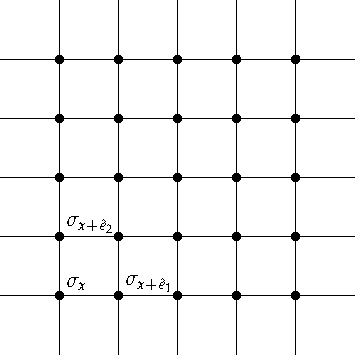
\includegraphics[]{Images/fig-2DIsing.pdf}
    
    \caption{2D Ising model on a square lattice. The spins sit on the nodes/crossings of the lattice, with interaction between neighbouring spins ($\mu = \pm \hat{e}_1, \pm \hat{e}_2$).}
    \label{fig-2DIsing}
\end{figure}

Typically we work in the thermodynamic limit where the lattice is very large (in this limit the boundary conditions should not be important to understand the physics, but this is something we can check). Writing down the Hamiltonian, we have:
\begin{equation}
    H_{interaction} = -J \sum_{x, \mu}\sigma_{x}\sigma_{x+\mu}
\end{equation}
Where $\mu$ runs over the vectors that point to the nearest neighbours of $x$ (so $x + \mu$ runs over the nearest neighbours of $x$). We will not concern ourselves too much with the lattice constant (we can just set it to one). Note that $\sigma_x\sigma_{x+\mu}$ is minimized if the two spins align, (as then $\sigma_x\sigma_{x+\mu}$ is positive and hence the negative sign out front gives the term a negative contribution). We can change the nearest neighbours assumption to include next nearest neighbours, infinite range etc. (and we can also change the behaviour of the interactions) but realistic interactions are short range so for now nearest neighbours is good to consider.

This is almost the Ising model; we can also add a coupling term to an external magnetic field:
\begin{equation}
    H_{B} = -B\sum_x \sigma_x
\end{equation}
where the spins will want to align with $B$ so as to lower the energy. So the Ising Hamiltonian is:
\begin{equation}
    H = H_{interaction} + H_{B} = -J \sum_{x, \mu}\sigma_{x}\sigma_{x+\mu} - B\sum_x \sigma_x.
\end{equation}
This simple two-parameter ($J, B$) model is already quite interesting. From it we will learn about universality - phase transitions tend to be the same for a large number of microsystems, e.g. the critical behavior for the Ising model and for liquid gas phase transition is the same. So this is why we can get away with studying something so simple.

\subsection{Analyzing the Ising Model - Phase Diagram Boundaries}
What we would like to compute is the partition function:
\begin{equation}
    Z = \sum_{\text{spins}}e^{-H/k_B T}
\end{equation}
and we would then like to calculate the free energy $F$, which is a function of the temperature $T$, the field $B$, and the number $N$:
\begin{equation}
F[T, B, N] = -k_B T \ln Z
\end{equation}
if we can find $F$, we can get all sorts of physical quantities, e.g. magnetization, susceptibility etc. For example we have the magnetization (average sum over all spins):
\begin{equation}\label{eq-magnetization}
    M = \left.-\dpd{F}{B}\right|_{N, T} = \frac{\sum_{\text{spins}}(\sum_x \sigma_x)e^{-H/k_B T}}{Z}
\end{equation}

As mentioned previously, we will assume that $N \to \infty$ (thermodynamic limit). What is left in our free energy is $T$ and $B$. So, we can draw a phase diagram:

\begin{figure}[htbp]
    \centering
    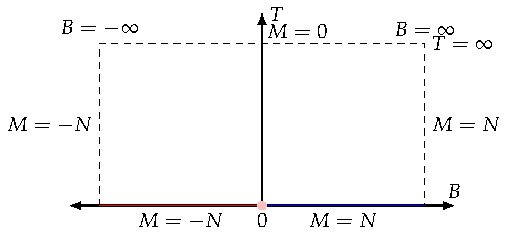
\includegraphics{Images/fig-Isingphasediagramboundaries.pdf}
    
    \caption{Phase Diagram Boundaries for the Ising Model, plotting temperature $T$ and magnetization $M$. As $B = \pm \infty$, the spins want to align all upwards ($M = N$)/downwards ($M = -N$) respectively. As $T \to \infty$, all configurations are equally likely and so $M = 0$. At $T = 0$, all spins aligning minimizes the energy and so for $B < 0$ we have $M = -N$ and for $B > 0$ we have $M = N$. At $T = 0, B = 0$ there is a first order phase transition.}
    \label{fig-Isingphasediagramboundaries}
\end{figure}

Note that as $T \to \infty$, we would first notice that our lab had burned down, but before that we would also notice that our material is no longer a ferromagnetic; it is a paramagnet with $M = 0$. We can see this from our expression for $M$ in Eq. \eqref{eq-magnetization}, where if $T \to \infty$ then $e^{-H/k_B T} = 1$ and so the up and down spins have equal weight, so the net summation comes out to zero.

At $B = \pm \infty$, we have $M \neq 0$. Specifically, if $M = \infty$ then all the spins want to align upwards so $M = N$ and if $M = -\infty$ then the spins want to align downwards so $M = -N$. As the temperature goes to zero, we are interested in the lowest energy state of the Hamiltonian. As all the spins are aligned, this minimizes the energy so actually we find $M = -N$ for all $B < 0, T = 0$ and $M = N$ for all $B > 0, T = 0$. What happens then at $B = 0$? We have a phase transitions between the two domains. We have a first order phase transition there where the magnetization completely flips.

What does the order of the phase transition mean? It refers to the number of the derivatives we can take of the free energy before the derivative does not exist. Here (at $T = 0$), $M = \text{sign}(B) N$, and the derivative of this does not exist at $B = 0$; so the first derivative of $F$ exists but the second one does not, so it is a first order phase transition. This comes from the Landau classification of phase transitions. This is not the full story; we have discovered many topological phases in recent times, and it could be argued that the classification of phases is not yet complete. If we integrate, at $T = 0$ we find $F = J\abs{B}$; this is continuous but not differentiable so the phase transition is first order.

\begin{figure}[htbp]
    \centering
    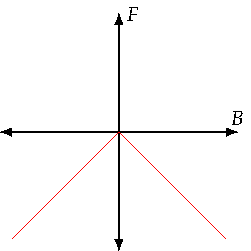
\includegraphics{Images/fig-FT0Ising.pdf}
    
    \caption{Plot of $F$ at $T = 0$ as a function of $B$. The free energy is continuous but not differentiable, and hence there is a first-order phase transition at $B = 0$. The slope of the free energy is $-J/J$.}
    \label{fig-FT0Ising}
\end{figure}

\subsection{Analyzing the Ising Model - $B = 0$ and Spontaneous Symmetry Breaking}
The line of $B = 0$ is interest. This is because the Hamiltonian has more symmetry in this case; namely the symmetry of flipping every $\sigma_x \leftrightarrow -\sigma_x$, or a $\mathbb{Z}_2$ symmetry (which can be represented, e.g. as $\set{1, -1}$ with multiplication). The magnetic field breaks this symmetry.

Note that if we are at some point in the right half of the phase diagram and we do a $\mathbb{Z}_2$ transformation, we map to the point on the other (left) side of the phase diagram (so on the $B = 0$ axis, we do not move at all!) Note however we cannot use symmetry to conclude that $M = 0$ at $B, T = 0$; as the magnetic moment here is dependent on the prior history of the system (how was this critical point reached). So we have some strange behaviour here; at this point, the Hamiltonian has $\mathbb{Z}_2$ symmetry but the actual state of the system does not inherit this symmetry; the system chooses one of the totally magnetized states depending on the prior history. This is known as \emph{spontaneous symmetry breaking}.

Now we can ask; if we go up the $B = 0$ axis (by turning on the temperature) from the $B, T = 0$ point, what happens? Does the symmetry remain broken? In the 1-D Ising model, there is a phase transition where the symmetry is unbroken; the magnetization goes back to $M = 0$. We will show that this comes about through solving the model. In higher dimensions, we cannot exclude the possibility that $M \neq 0$ persists for a while even as we turn up $T$; for example it might be possible that $M$ decays up to some point after hitting zero. We then have a discontinuity in the phase diagram partially along the $T = 0$ axis. We have a line of first order phase transitions, and it ends at some point in a second order phase transition. Unlike the boundaries of the diagrams, we have not really justified this statement; we will have to return to its proof later. 

\begin{figure}[htbp]
    \centering
    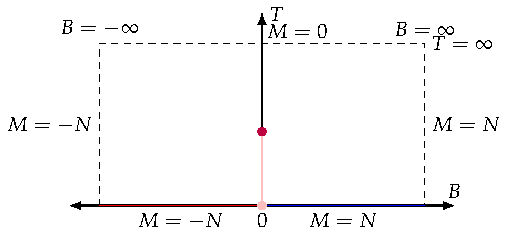
\includegraphics{Images/fig-IsingphasediagramB0.pdf}
    \caption{For dimensions larger than 1, $M \neq 0$ persists at $B = 0$ even as the temperature is tuned up. This results in a ``first order phase transition line'' partway up the $B = 0$ axis, culminating in a second order phase transition point.}
    \label{fig-IsingphasediagramB0}
\end{figure}

It is difficult to study the phase transitions in generality, so we will (later) focus our attention to the point around the second order phase transition. Specifically, things are complicated by the magnetic field, so we will study a neighbourhood of the second order phase transition that lies on the $B = 0$ axis.

We will be able to study the 1-D model in full generality, but this is not very interesting as the ``phase transition line'' we see above will get shrunk to a point. The 2-D model has been solved but only at $B = 0$. 

\subsection{Solving the 1-D model}
One of the slightly unsatisfying things about the study of this system is that the models in different dimensions have different ad-hoc ways of solving them analytically. When we start to look at approximations, we will see a unifying formalism (e.g. renormalization group).

We consider the 1-D Ising model, which is just a chain of classical spins. 

\begin{figure}[htbp]
    \centering
    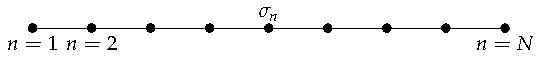
\includegraphics{Images/fig-1DIsing.pdf}
    \caption{Cartoon of 1D Ising model (pictured with $N = 9$ spins). The spin at site $n$ is denoted $\sigma_n$.}
    \label{fig-1DIsing}
\end{figure}

The Hamiltonian takes the form:
\begin{equation}
    H = -H\sum_{n=1}^{N-1}\sigma_n \sigma_{n+1} - B\sum_n \sigma_n
\end{equation}
The route to the solution here is just a brute-force calculation of the partition function:
\begin{equation}
    Z = \sum_{\sigma_1 = \pm 1, \ldots, \sigma_n = \pm 1} e^{\frac{J}{k_B T}\sum_n \sigma_n \sigma_{n+1} - \frac{B}{k_B T}\sum_{n}\sigma_n}
\end{equation}
we rewrite this as an extended multiplication:
\begin{equation}
    Z = \sum_{\sigma_1 = \pm 1} \sum_{\sigma_2 = \pm 1} \ldots \sum_{\sigma_n = \pm 1}e^{-\frac{B}{2k_B T}\sigma_1}\left[e^{\frac{J}{k_B T}\sigma_1 \sigma_2 - \frac{B}{2k_B T}(\sigma_1 + \sigma_2)}\right]\left[e^{\frac{J}{k_B T}\sigma_2 \sigma_3 - \frac{B}{2k_B T}(\sigma_2 + \sigma_3)}\right] \ldots \left[e^{\frac{J}{k_B T}\sigma_{N-1} \sigma_N - \frac{B}{2k_B T}(\sigma_{N-1} + \sigma_N)}\right]e^{-\frac{\beta}{2k_B T}\sigma_N}
\end{equation}
Why would we do this? Because we can take the objects inside the square brackets and call it a 2x2 matrix $T_{ab}$ (with elements that depend on whether the spins are up or down):
\begin{equation}
    T_{ab} = e^{\frac{J}{k_B T}\sigma_a \sigma_b - \frac{B}{2k_B T}(\sigma_a + \sigma_b)}
\end{equation}
where $T_{11}$ has $\sigma_a = \sigma_b = 1$, $T_{22}$ has $\sigma_a = \sigma_b = -1$ and so on. Explicitly:
\begin{equation}
    T_{ab} = \m{e^{\frac{J-B}{k_B T}} & e^{-\frac{J}{k_B T}} \\ e^{-\frac{J}{k_B T}} & e^{\frac{J + B}{k_B T}}}
\end{equation}
We can then write the partition function as:
\begin{equation}
    Z = \sum_{\sigma_1 = \pm 1}\sum{\sigma_N = \pm 1} e^{-\frac{B}{2k_B T}\sigma_1}(T^{N-1})_{\sigma_1\sigma_N} e^{-\frac{B}{2k_B T}\sigma_N}
\end{equation}
what does this buy us? Because $T_{ab}$ is real and symmetric, it can be diagonalized by a similarity transform. So, $T$ can be written as:
\begin{equation}
    T = R\Lambda R^T = \m{\cos\theta & -\sin\theta \\ \sin\theta & \cos\theta}\m{t_+ & 0 \\ 0 & t_-}\m{\cos\theta & \sin\theta \\ -\sin\theta & \cos\theta}
\end{equation}
with $R$ rotation matrices. The partition function then becomes:
\begin{equation}
    Z = \sum_{\sigma_1 = \pm 1, \sigma_N = \pm 1} e^{-\frac{B}{2k_B T}\sigma_1}R\m{t_+^{N-1} & 0 \\ 0 & t_-^{N-1}}R^T e^{-\frac{B}{2k_B T}\sigma_N}
\end{equation}
where we have used that $RR^T = R^TR = \mathbb{I}$ and so all but the first and last rotation matrices cancel. 

Now, what happens here? Since $N$ we take to be large, one of the eigenvalues will grow much more and will dominate. If we are interested in taking a logarithm of $Z$ and choosing the part that grows like $N$, we can just look at the larger eigenvalue. We don't really have to calculate the details if we just figure out what the larger of the two eigenvalues of the transfer matrix is; we can just consider:
\begin{equation}
    F = -k_B T N \ln t_+.
\end{equation}
But we are out of time, so we leave this to next class...

\newpage
\section{The 1-D Ising Model, Continued}
Recall we were studying the 1D Ising Hamiltonian:
\begin{equation}
    H = -\sum_{n=1}^{N-1}J\sigma_n \sigma_{n+1} - B \sum_{n=1}^N \sigma_n.
\end{equation}
This is one of the few exactly solvable cases with a nonzero external $B$ field. All of the other famous solvable Ising models have the $B$-fields turned off. Note that solving the 1-D case is really easy (left as an exercise) if $B = 0$. With $B \neq 0$, we use a transfer matrix technique that we finish today.

Last class we also studied the phase diagram of the Ising model; we considered the boundaries of the phase diagram, though the central areas were left undetermined. In 1D the center of this phase diagram is not very interesting at all (and no interesting phase transition is really observed) but it is still valuable to consider to get used to the model and to explore the analytical techniques to solve it.

\subsection{Large-field case}

Note that in the case where $B \gg J$, the partition function is very simple as we can neglect the exchange/$J$ term in the energy:
\begin{equation}
    Z = \sum_{\sigma_n} \prod_n e^{\frac{B}{k_B T}\sigma_n} = \left(2\cosh\frac{B}{k_B T}\right)^N
\end{equation}
so:
\begin{equation}
    F = -k_B T \ln Z = -k_B T N \ln (2\cosh\frac{B}{k_B T})
\end{equation}
with magnetization per spin:
\begin{equation}
    m = \frac{M}{N} =  \frac{\left.-\dpd{F}{B}\right|_{N, T}}{N} = \tanh(\frac{B}{k_B T})
\end{equation}
which is $\pm 1$ (i.e. full magnetization upwards/downwards) as $B \to \pm \infty$. 

\subsection{The Transfer Matrix and Solving 1-D Ising Model}
We recall we found the transfer matrix:
\begin{equation}
    T_{ab} = \m{e^{\frac{J + B}{k_B T}} & e^{-\frac{J}{k_B T}} \\ e^{-\frac{J}{k_B T}} & e^{\frac{J + B}{k_B T}}}
\end{equation}
and with this we were able to express the partition function for the (general) 1-D Ising model partition function as:
\begin{equation}
    Z = \m{e^{\frac{B}{2k_B T}} & e^{-\frac{B}{2k_B T}}} T^{N - 1}\m{e^{\frac{B}{2k_B T}} \\ e^{-\frac{B}{2k_B T}}}
\end{equation}
we used open boundary conditions here; but it would also be possible to fix the orientations of spins at the edges of the chain, or to use periodic boundary conditions where we identify the first and last spin of the chain. In the limit of large $N$, the boundary conditions are not relevant and the boundary conditions do not matter.


So how do we go about analyzing this partition function? Well, $T_{ab}$ is a real symmetric matrix. A real symmetric matrix can be diagonalized via a similarity transformation:
\begin{equation}
    T = R\Lambda R^T = \m{\cos\theta & -\sin\theta \\ \sin\theta & \cos\theta}\m{t_+ & 0 \\ 0 & t_-}\m{\cos\theta & \sin\theta \\ -\sin\theta & \cos\theta}
\end{equation}
Then, since $RR^T = \mathbb{I}$ it follows that:
\begin{equation}
    T^{N-1} =  \m{\cos\theta & -\sin\theta \\ \sin\theta & \cos\theta}\m{t_+^{N-1} & 0 \\ 0 & t_-^{N-1}}\m{\cos\theta & \sin\theta \\ -\sin\theta & \cos\theta}
\end{equation}
Now we study this when $N$ is large; then the partition function is dominated by the larger eigenvalue $t_+$; we can keep terms of $O(N)$ and throw away terms of $O(1)$. We thus come to the conclusion:
\begin{equation}
    F = -k_B T N\ln t_+.
\end{equation}
Now if we wanted to find this free energy explicitly and confirm this assertion that the larger eigenvalue dominates, we could also explicitly solve this system. For this, the periodic boundary conditions may be easiest, as we can just take the trace of $T^{N-1}$ (and we don't get any boundary terms).

Solving for the eigenvalues of $T$, we find:
\begin{equation}
    t_\pm = e^{\frac{J}{k_B T}}\cosh\frac{B}{k_B T} \pm \sqrt{e^{\frac{2J}{k_B T}}\sinh^2\frac{B}{k_B T} + e^{-\frac{-2J}{k_B T}}}
\end{equation}
which we note are both real and positive. The free energy is then:
\begin{equation}
    F = -k_B T\ln t_+^N = -N J - k_B T N\ln\left[\cosh\frac{B}{k_B T} + \sqrt{\sinh^2\frac{B}{k_B T} + e^{-\frac{4J}{k_B T}}}\right]
\end{equation}
here $-NJ$ is very much like a ``zero point energy''. If we look at the limits of this expression, this matches up with the boundaries of the phase diagram that we analyzed previously! (we can find the magnetization $M = \left.\pd{F}{B}\right|_{N, T}$ and then see that it reproduces our predictions in the $T \to 0/\infty$ and $B \to \pm \infty$ limits). We also note that $F$ is completely non-singular in the inside of the phase diagram, and with the exception at $F = 0, B = 0$ it is also completely non-singular on the boundaries of the phase diagram.

At that point, we cannot use symmetry to conclude that the magnetization is $M = 0$; instead it is history dependent. It is highly ambiguous, and the symmetry is spontaneously broken there.

\subsection{Correlation Functions}
So, we've solved for the thermodynamics of the system! But another line of interest in studying spin systems are correlation functions.

To start, consider $\avg{\sigma_x}$ (one-point correlation function). If we have periodic BCs, then this is site independent and furthermore just gives the magnetization per spin and so:
\begin{equation}
    \avg{\sigma_x} = m
\end{equation}
but if there are other BCs, then we need to take into account corrections:
\begin{equation}
    \avg{\sigma_x} = m + \text{boundary corrections}
\end{equation}
we can explicitly evaluate $\avg{\sigma_x}$ are using the transfer matrix formalism. E.g. for the case of open boundary conditions:
\begin{equation}
    \avg{\sigma_x} = \frac{\m{e^{\frac{B}{2k_B T}} & e^{-\frac{B}{2k_B T}}} T^{x-1} \m{1 & 0 \\ 0 & -1} T^{N - x} \m{e^{\frac{B}{2k_ B T}} \\ e^{-\frac{B}{2k_B T}}}}{Z}
\end{equation}
Now in principle we could evaluate this. We skip this as this is not particularly illuminating. With periodic BCs, we get rid of the boundary terms and just take the trace:
\begin{equation}
    m = \frac{\Tr\left[ T^{x-1} \m{1 & 0 \\ 0 & -1} T^{N - x}\right]}{\Tr T^{N-1}} = \frac{\Tr\left[ T^{N-1} \m{1 & 0 \\ 0 & -1}\right]}{\Tr T^{N-1}} = \frac{c_+t_+^{N-1} - c_-t_-^{N-1}}{c_+t_+^{N-1} + c_-t_-^{N-1}}
\end{equation}
where we have used the cyclicity of the Trace; $\Tr(ABC) = \Tr(CAB) = \Tr(BCA)$. 

There are then higher-point correlation functions. We consider the two-point correlation function (which already give us some interesting information):
\begin{equation}
    \avg{\sigma_x \sigma_y}
\end{equation}
but actually the connected correlation function will be a little more interesting to study:
\begin{equation}
    \avg{\sigma_x \sigma_y} - \avg{\sigma_x}\avg{\sigma_y}
\end{equation}
this in principle again we can evaluate for any boundary condition, but again let's just look at the simplest case of the periodic BCs. Then:
\begin{equation}
    \avg{\sigma_x\sigma_y} = \frac{\Tr\left[T^{x-1}\pauliz T^{y-x} \pauliz T^{N-y}\right]}{\Tr T^{N-1}}
\end{equation}
and $\avg{\sigma_x}$ is independent of $x$/the site, so $\avg{\sigma_x}\avg{\sigma_y} = \avg{\sigma_x}^2$ and so:
\begin{equation}
    \avg{\sigma_x \sigma_y} - \avg{\sigma_x}\avg{\sigma_y} = \frac{\Tr\left[T^{x-1}\pauliz T^{y-x} \pauliz T^{N-y}\right]}{\Tr T^{N-1}} -  \left(\frac{\Tr\left[ T^{x-1} \m{1 & 0 \\ 0 & -1} T^{N - x}\right]}{\Tr T^{N-1}}\right)^{2}
\end{equation}

Now we can plug in the diagonal form of $T$ and evaluate all of this; at the end of the day\footnote{I take home my hard earned pay all alone\ldots} we end up with:

\begin{equation}
    \avg{\sigma_x \sigma_y} - \avg{\sigma_x}\avg{\sigma_y} = \frac{t_+^{y-x}t_-^{N-1-(y-x)} + t_-^{y-x}t_+^{N-1-(y-x)}}{t_+^{N-1} + t_-^{N-1}}
\end{equation}
Now we notice a symmetry; the connected correlation function only depends on the distance from $y$ to $x$, but not the actual sites themselves! Now, if we assume that the sites $y, x$ are sufficiently close, i.e. we work in the limit:
\begin{equation}
    N \gg (y - x) \geq 1
\end{equation}
the above simplifies to:
\begin{equation}
    \avg{\sigma_x \sigma_y} - \avg{\sigma_x}\avg{\sigma_y} \approx \left(\frac{t_-}{t_+}\right)^{y-x} = e^{-\abs{x-y}/\xi}
\end{equation}
where $\xi$ is the \emph{correlation length}. To get this correlation length, we can take a logarithm of both sides:
\begin{equation}
    \xi = \frac{1}{\ln(t_+/t_-)}
\end{equation}
which we can then find explicitly by plugging in the form of the eigenvalues.

\subsection{The 1-D Ising Model is Disordered at Finite Temperature}
Landau gives the following argument for why the Ising model is always disordered in one dimension, that is to say, why is $m = 0$ in 1-D on the $B = 0$ line for all $T> 0$. 

\begin{figure}[htbp]
    \centering
    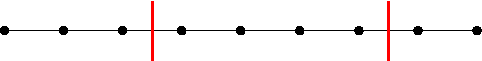
\includegraphics{Images/fig-1DIsingdisorder.pdf}
    \caption{Cartoon of the setup for Landau's argument for disorder in the 1D Ising model. We consider flips in the bonds between spins (domain walls) in the chain of spins.}
    \label{fig-1DIsingdisorder}
\end{figure}

The Hamiltonian is minimized if all spins are aligned. The next lowest energy state is one where there is a single flipped spin. Compared to the lowest energy state, this has energy penalty $-2J$ and so has a boltzmann factor $e^{-2J/k_B T}$ that suppresses the probability of this happening. So up to an overall factor $e^{JN/k_B T}$ which takes into account the zero point energy, the first twoo terms in the partition function (the low-$T$ expansion) is:
\begin{equation}
    Z \sim 1 + Ne^{-2J/k_B T}
\end{equation}
with the $N$ appearing as these are the possible bonds (domain walls) between spins that could be flipped. Then we add the next term for 2 flips, which yields:
\begin{equation}
    Z \sim 1+ Ne^{-2J/k_B T} + \binom{N}{2}e^{-4J/k_B T}
\end{equation}
and in general the term with $n$ flipped bonds has coefficient $\binom{N}{n}$ and so:
\begin{equation}
    Z \sim 1 + Ne^{-2J/k_B T} + \binom{N}{2}e^{-4J/k_B T} + \ldots + \binom{N}{n}e^{-2nJ/k_B T} + \ldots
\end{equation}
now, if we look at the most likely distribution, we see that the $n = N/2$ unmagnetized state is favoured. The entropy grows faster than the number of bonds, vs. the energy grows proportionally than the number of bonds; so the entropy wins out and we see that the unmagnetized state is favoured.

Why does this argument fail in higher dimensions? Because the domain walls scale differently in 2D. The entropy grows as the number of closed paths (rather than as the number of points on the line) which means that the above argument does not apply in the same way (and we do get a phase transition in higher dimensions)!

Lots of cool stuff that Ising models can be tied to... e.g. Majorana fermions in 2D, random surface theories, fermionic string theories in 3D...

\subsection{Teaser - Infinite Range Ising Model}
We look at another analytically solvable Ising model. Here, we remove the restriction that the spins only interact with their nearest neighbours. Specifically, we consider the case where every spin interacts with every other spin with the same interaction strength. While this is not at all a physically realistic system (because interactions are not infinite range in real life, of course) but we will see that the phase diagram of this model is more interesting, with phase transitions occuring at finite $T$ across $B = 0$. 

Our Hamiltonian is:
\begin{equation}
    H = -\frac{J}{N}\sum_{n, n'}\sigma_n \sigma_{n'} - B\sum_n \sigma_n
\end{equation}
where the sum $\sum_{n, n'}$ runs over all pairs of spins in the lattice. We are able to evaluate this by summing over one spin at a time (with each spin giving an equal contribution to the overall partition function), because all spins look the same here:
\begin{equation}
    Z = \sum_{\sigma_n} e^{\frac{J}{k_B T}\sum_{n, n'}\sigma_n \sigma_{n'} + \frac{B}{k_B T}\sum_n \sigma_n}
\end{equation}
This looks awful, but we can consider an analogy with a Gaussian integral. Consider:
\begin{equation}
    \int_{-\infty}^\infty dm e^{-\left(m - \frac{1}{N}\sum_x \sigma_x\right)^2\frac{JN}{k_B T}}
\end{equation}
We can solve this by translating the integral to get rid of $\sum_x \sigma_x$ which is a constant w.r.t. the variable of integration. The integral then evaluates to:
\begin{equation}
    \int_{-\infty}^\infty dm e^{-\left(m - \frac{1}{N}\sum_x \sigma_x\right)^2\frac{JN}{k_B T}} = \sqrt{\frac{k_B T}{NJ}\pi}
\end{equation}
So then:
\begin{equation}
    1 = \sqrt{\frac{NJ}{\pi k_B T}}\int_{-\infty}^\infty dm e^{-\left(m - \frac{1}{N}\sum_x \sigma_x\right)^2\frac{JN}{k_B T}}
\end{equation}
Now let us put this factor of 1 into the partition function. We will then see that terms cancel, and we get an integral that we can solve - if $N$ is large - using a saddle point integration technique. From this we can obtain the free energy and learn the thermodynamic properties of the system.

\end{document}